% To add an image or include a .tex file you need to add
% \CWD
% to the relative (to the main document) path.
%
% Example:

Um famoso (e antigo) desafio jogado nas ruas consiste em esconder uma bolinha abaixo de um dentre três copos e dizer onde a bolinha ficou após o desafiante trocar os copos de posição.

\begin{figure}[H]
  \centering
  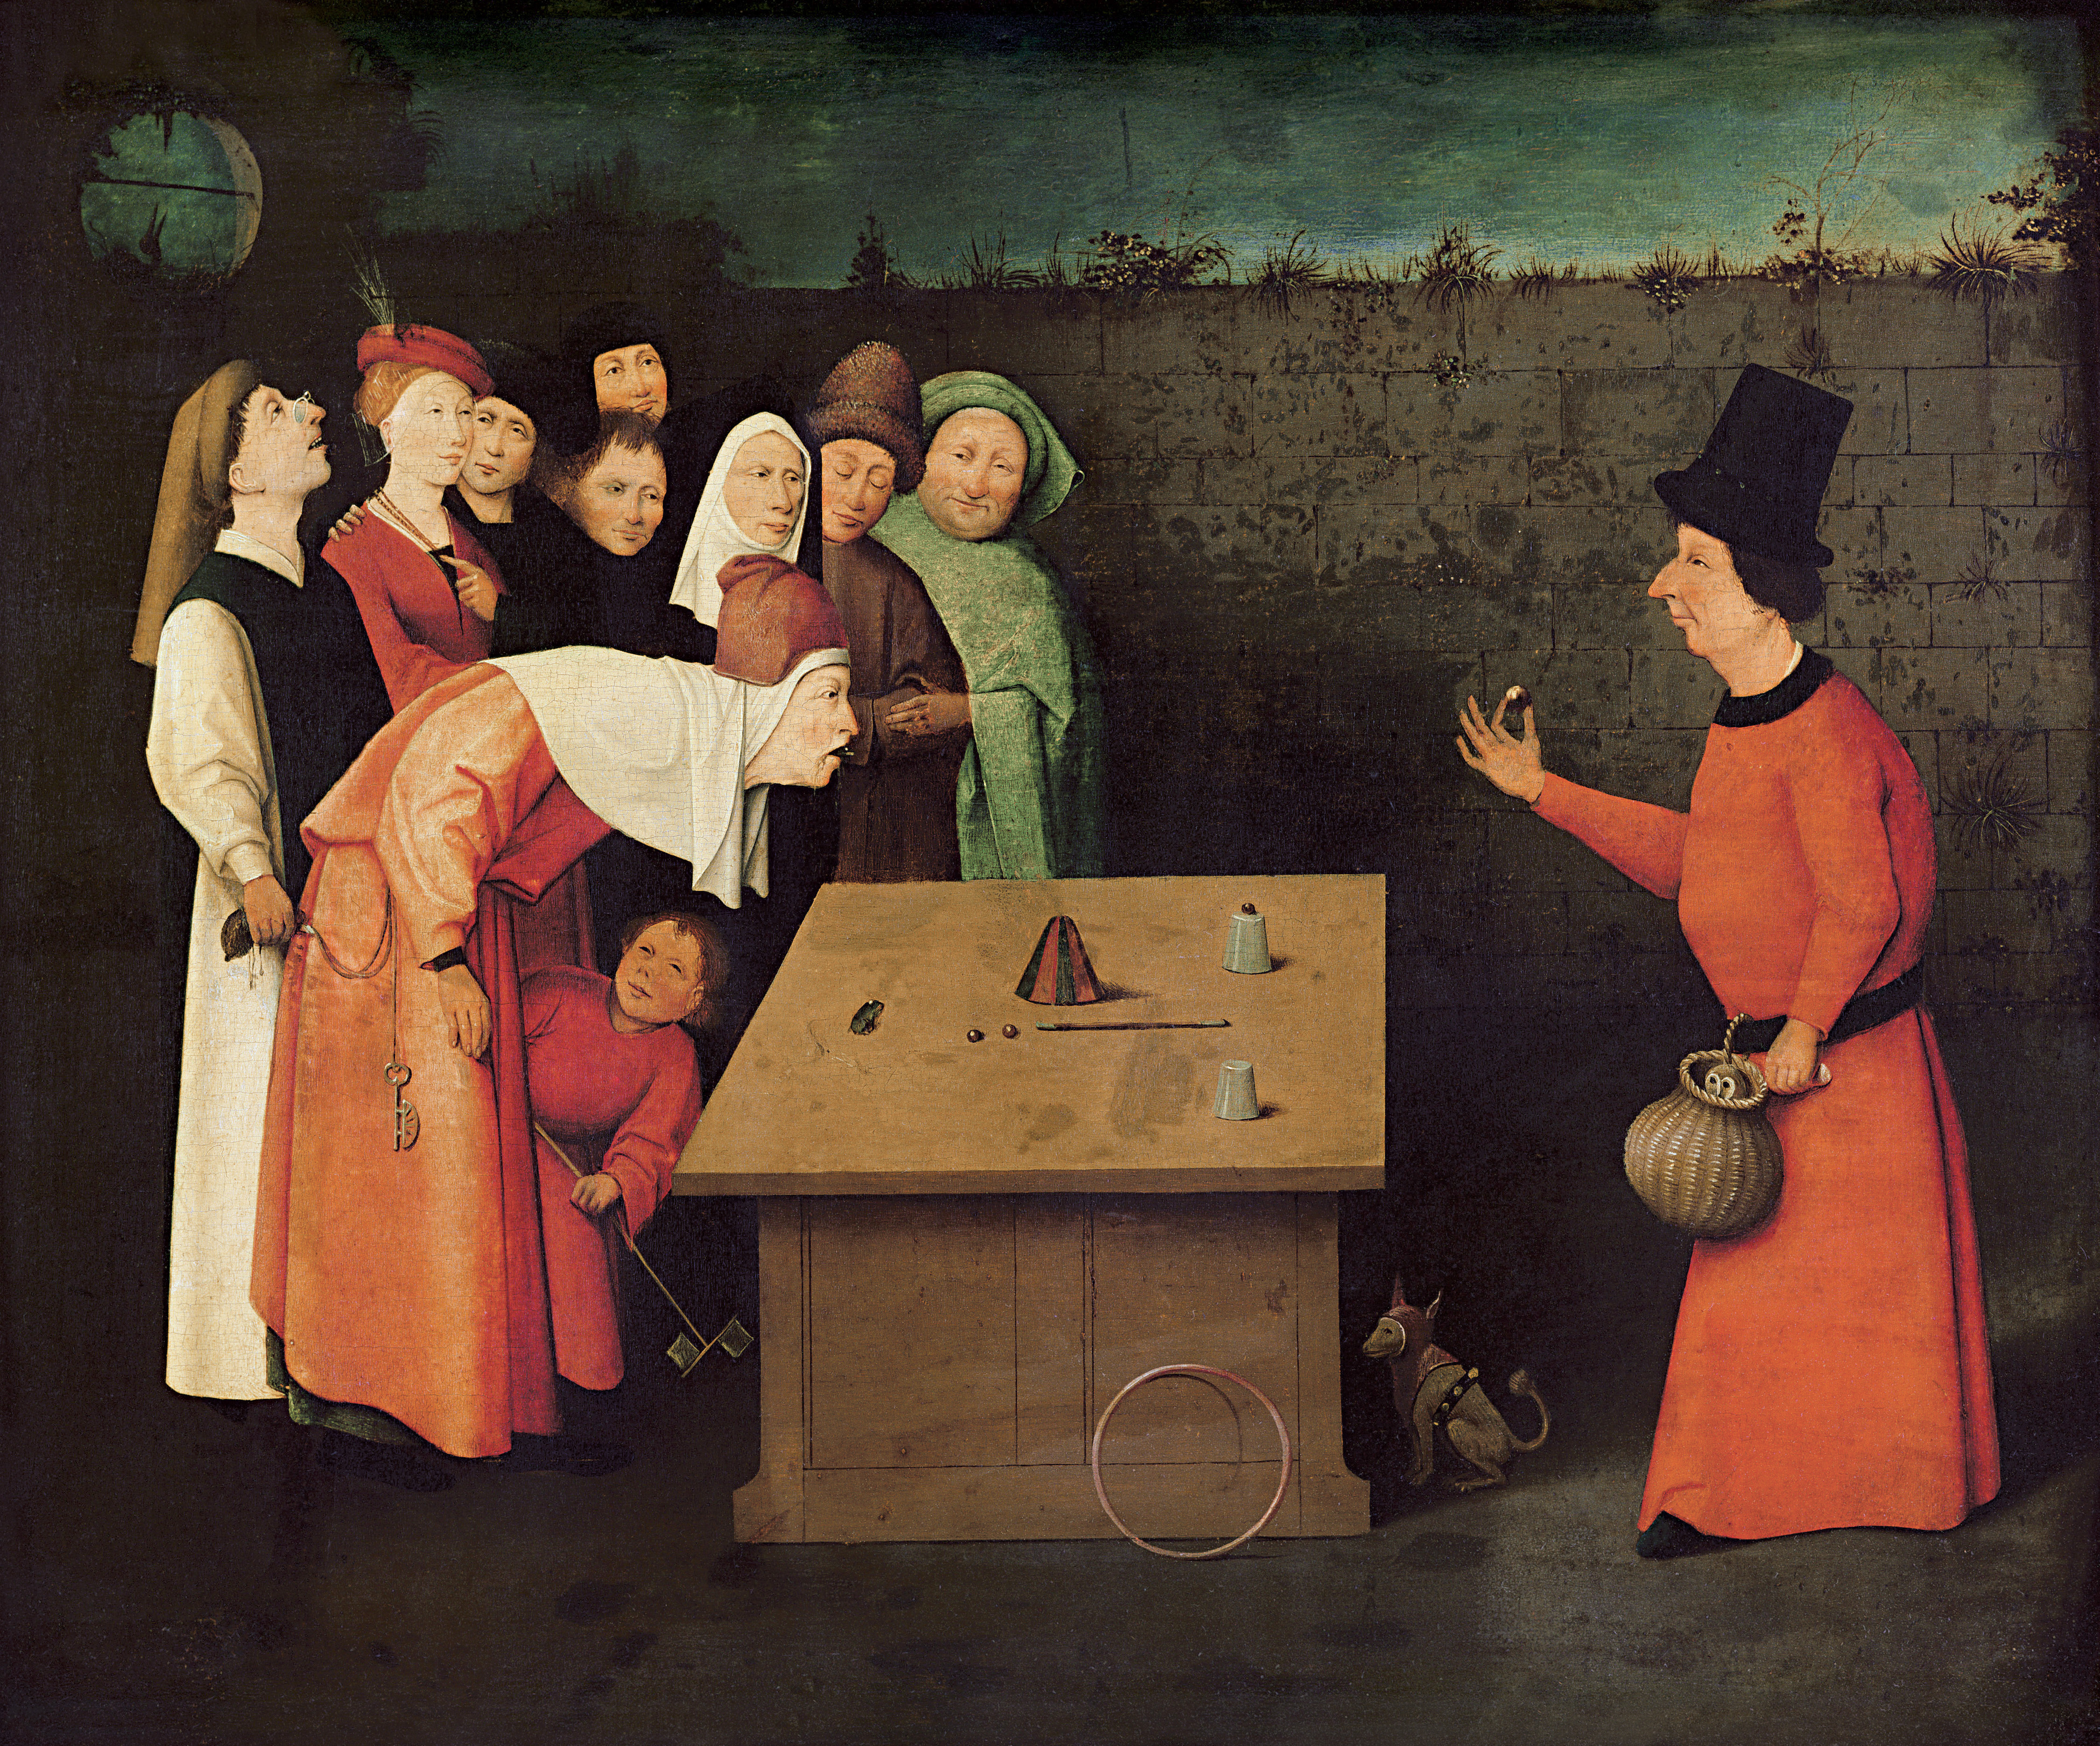
\includegraphics[width=5cm]{\CWD/jogo-medieval.jpg}
  \caption{Jogo da bolinha sendo jogado na era medieval.}
\end{figure}

Para garantir a vitória, os desafiantes costumam fazer movimentos muito rápidos. Entretanto, como você é esperto, você conseguiu ver todos os movimentos de ``troca'' dos copos. 

Dado que os copos são numerados de $1$ a $3$ e a bolinha começa no copo do meio (copo $2$), imprima qual é a posição final da bolinha após $N$ movimentos de troca de copos.

%
% For input, use one of the following
%

\section*{Entrada}

A primeira linha da entrada consiste em um inteiro $N$ tal que $1 \leq N \leq 2\times10^5$. Depois seguem $N$ linhas, cada uma contendo dois inteiros $A, B$ ($1 \leq A, B \leq 3$), que indica que o copo $A$ foi trocado com o copo $B$.

%
% For output, use one of the following
%

\section*{Saída}

A saída deve consistir de um número de $1$ a $3$: qual foi a posição final da bolinha.

\section*{Restrições}

\begin{itemize}
\item $1 \leq N \leq 2\times 10^5$.
\end{itemize}

%\sampleio will look for files named sample-n.in and sample-n.sol (where n is 1, 2, 3...)
%in the documents directory and include them as samples.

\exemplo
